\documentclass[draft,tec]{agutexSI2019}

\usepackage{graphicx}

\setkeys{Gin}{draft=false}

\begin{document}

\begin{article}

\section{Introduction}\label{sec:intro}

This supplement includes a description of the code, with a presentation of the features implemented followed by results of extensive benchmarks, implemented to verify that the code solves correctly a large range of problems (Table \ref{tab:list}).

The code is written in Fortran90 and uses the finite element method (FEM) with quadrilateral $Q_1P_0$ elements (continuous bilinear velocity and discontinuous constant pressure), associated with the direct solver MUMPS (see Section \ref{sec:solver}). Since $Q_1P_0$ elements do not satisfy Ladyzhenskaya, Babuska and Brezzi (LBB) stability condition \cite{Donea2003}, the elements are stabilised in postprocessing to avoid spurious pressures by means of a triple interpolation to smooth the pressure. Following this procedure, the elemental pressure is interpolated onto nodes, back onto elements and back again onto nodes (see Section \ref{sec:stokes}).

Elemental properties (density, viscosity, thermal conductivity, specific heat and thermal expansion) are related to the composition of each elemenet ,determined by means of Lagrangian markers. Each marker is characteristic of different materials in the domain. Therefore, elemental properties (with exception of the viscosity) is calculated using an arithmetic mean, as \[P_e=\frac{1}{n}\sum_{i=1}^n P_i\]
where $P_e$ is the elemental property, $P_i$ is the property characteristic of the material of each marker and $n$ is the number of markers of the element. Differently, the average scheme for the elemental viscosity can be chosen between harmonic, geometric and arithmetic mean. Markers can be placed regularly or randomly at the beginning of the simulation and their advection is performed by a 4th-order Runge-Kutta, interpolating the velocity field on each markers by means of the shape functions (see Section \ref{sec:runge}). During the simulation, each marker carries memory of temperature, pressure and accumulated strain, which are determined interpolating the nodal parameters, as for the velocities. The number of markers contained in each element is mantained between $n_{min}$ and $n_{max}$, which can be chosen by the user at the begininng of the simulation. When in an element there are less markers than $n_{min}$ the code adds random markers to reach the $n_{min}$, while if the number is higher than $n_{max}$ some of them are deleted. When new markers are added, they assume the properties of the nearest marker. In this way elements are never empty and mantain a number of markers inside a prefixed range.

The thermo-mechanics of crust-mantle systems can be described by means of the conservation of mass, momentum and energy equations, expressed as follows:
\begin{equation}\label{eq:mass}
\nabla \cdot \vec{u}=0
\end{equation}
\begin{equation}\label{eq:momentum}
-\nabla p + \nabla \cdot \vec{\tau} + \rho \vec{g} = 0
\end{equation}
\begin{equation}\label{eq:energy}
\rho C_p \left(\frac{\partial T}{\partial t} + \vec{u} \cdot \nabla T \right) = \nabla \cdot \left(K\nabla T\right) + H
\end{equation}

where $\vec{u}$ is the velocity, \textit{p} is the pressure, $\vec{\tau}$ is the deviatoric stress, $\rho$ is the density, $\vec{g}$ is the gravity acceleration, $C_p$ is the specific heat at constant pressure, \textit{T} is the temperature, \textit{K} is the thermal conductivity and \textit{H} is the total internal heat production. The deviatoric stress tensor can be write in terms of the strain rate tensor as $\vec{\tau}=2\mu\dot{\epsilon}$, with $\dot{\epsilon}=\frac{1}{2}\nabla\vec{v}$. Therefore, eq. \ref{eq:momentum} can be rewrite as:
\begin{equation}\label{eq:momentum_pressure}
-\nabla p + \nabla \cdot \left(\mu \nabla \vec{v}\right) + \rho \vec{g} = 0
\end{equation}
The penalty method has been implemented in order to enforce incompressibility, so that eq. \ref{eq:mass} can be write as:
\begin{equation}\label{eq:mass_penalty}
\nabla \cdot \vec{u} + \frac{p}{\lambda}=0
\end{equation}
where $\lambda$ is the so-called penalty parameter, which should be 6-7 orders of magnitude larger than the shear viscosity to ensure that mass conservation is satisfied \cite{Donea2003,Thieulot2014}. To support large viscosities variations the penalty parameter has been related to the effective elemental viscosity by means of a dimensionless coefficient, so that $\lambda=\lambda_e(e)\mu_{eff}(e)$ \cite{Marotta2006,Dabrowski2008,Thieulot2014}. Finally, using pressure from eq. \ref{eq:mass_penalty}, eq. \ref{eq:momentum_pressure} can be rewrite as:
\begin{equation}\label{eq:momentum_penalty}
\lambda \nabla \left(\nabla \cdot \vec{v} \right) + \nabla \cdot \left(\mu \nabla \vec{v}\right) + \rho \vec{g} = 0
\end{equation}
Results of benchmarks performed to verify the correctness in the immplementation of eqs. \ref{eq:momentum_penalty} and \ref{eq:energy} are shown in Section \ref{sec:momentum}. To strengthen the penalty method, it has been associated to the iterative Uzawa method, as described in detail in \citeA{Dabrowski2008} and \citeA{Thieulot2014} (see Section \ref{sec:poiseuille}). The stabilisation of the advection term of the energy equation (eq. \ref{eq:energy}) needed to avoid possible oscillations in the thermal solution in case where advection dominates over diffusion, has been implemented by means of a streamline-upwind Petrov–Galerkin (SUPG) method, for which the shape functions in the advection term are modified to have
\[(\textbf{N}^*)^T=\textbf{N}^T + \tau \vec{v} \textbf{B}\]
The choice of parameter $\tau$ follows the discussion in \citeA{Thieulot2011} and \citeA{Thieulot2014} (see Section \ref{sec:advection}).

\!!!!!!! Marcatori Lagrangiani e accennare a tutto  After the last interpolation, nodal pressure is used to determine pressure onto each Lagrangian marker.

\section{Solver}\label{sec:solver}
MUMPS (MUltifrontal Massively Parallel Solver) is a software package for solving systems of linear equations of the form $A \cdot x = b$, where \textit{A} is a square sparse matrix, by means of a direct method. Correctness of the solution and performances of the solver in terms of time and memory usage have been tested solving the Stokes flow with the analytical solution proposed by \citeA{Donea2003}.

\subsection{Stokes flow}\label{sec:stokes}
The problem consists of determining velocity field $(u,v)$ and pressure $p$ in case of prescribed body forces:
\[b_1=(12-24y)x^4+(-24+48y)x^3+(-48y+72y^2-48y^3+12)x^2+(-2+24y-72y^2+48y^3)x+1-4y+12y^2-8y^3\]
\[b_2=(8-48y+48y^2)x^3+(-12y+72y-72y^2)x^2+(4-24y+48y^2-48y^3+24y^4)x-12y^2+24y^3-12y^4\]
for which the exact solution is:
\[u(x,y)=x^2(1-x)^2(2y-6y^2+4y^3)\]
\[v(x,y)=-y^2(1-y)^2(2x-6x^2+4x^3)\]
\[p(x,y)=x(1-x)\]
The domain is a square with $L_x=L_y=1$ and a constant viscosity ($\mu=1$). Velocities are set to no slip conditions $(\vec{v}=0)$ on all boundaries. The problem has been performed for different grid resolution (between 8x8 and 1024x1024 elements).

Fig. \ref{fig:errors} shows that both velocity field and pressure converge to the exact solution with the decrease of the element size, following the theoretical convergence rate. The convergence of pressure, in contrast with the observation by \citeA{Donea2003} for $Q_1P_0$ elements, indicate the effectiveness of the smoothing procedure. Solve times and memory usage needed to generate the solution are shown in Fig. \ref{fig:MUMPS}.

\section{Momentum and energy equations}\label{sec:momentum}
Benchmarks in this Section show the accomplishment of the mass conservation equation with the Uzawa method (Poiseuille flow benchmark), the correctness of the solution of the momentum and energy equations (Instantaneous 2D Stokes sphere, Rayleigh-Taylor, mantle convection and thin-layer experiments), and the functionality of the stabilisation of the advection term in the energy equation.

\subsection{Poiseuille flow}\label{sec:poiseuille}
The domain is a rectangle with $L_x=2$ and $L_y=1$ and constant density and viscosity ($\rho=1$ and $\mu=1$), gravity acceleration $\vec{g}=0$ and penalty parameter $\lambda=10^8$. The grid is composed by 40×20 elements. Velocities are set to no slip conditions $(\vec{v}=0)$ at the top and the bottom, and a parabolic profile is imposed on the sides, with $u=y(1-y)$ and $v=0$.

The velocity field predicted by the model follows the expected parabolic profile (Fig. \ref{fig:poiseuille}a) and, in case of the classic penalty method with no iterations, the pressure is clearly related to the divergence by means of the penalty parameter (Fig. \ref{fig:poiseuille}b and c). Fig. \ref{fig:poiseuille}d shows that one iteration is sufficient to bring the divergence down to $10^{15}$, with no correlation with the pressure field.

\subsection{Instantaneous 2D sphere}\label{sec:ist_sphere}
The domain is a square with $L_x=L_y=1$ and gravity $g=(0,-1)$. The fluid has constant density and viscosity ($\rho_f=1$ and $\mu_f=1$). The sphere is in the middle of the domain with a radius R = 0.123456798 and has constant density and viscosity ($\rho_s=1.01$ and $\mu_s=10^3 \cdot \mu_f$).
Velocities are set in order to distinguish three cases:
\begin{enumerate}
\item FS: free slip conditions on all sides.
\item NS: no slip conditions on all sides.
\item OT: free slip conditions on the sides and the bottom, and open boundary at the top.
\end{enumerate}
All the three cases have been performed for different frid resolutions (between 16x16 and 512x512 elements) and with harmonic, geometric and arithmetic averages for the viscosity. The solutions generated in terms of the velocity ($v_{rms}$, $u_{min}$, $u_{max}$, $v_{min}$, $v_{max}$, $\vec{v}(0.5;0.5)$) and pressure ($p_{min}$, $p_{max}$, $p_{avg}$) fields have been compared with solutions generated by ASPECT.

\subsection{Rayleigh-Taylor instability}\label{sec:rayleigh}
This problem has been performed as the isoviscous case (Case 1a) originally presented by \citeA{vanKeken1997}. The domain has $L_x=0.9142$ and $L_y=1$ and gravity $g=(0,-1)$. Two fluids with same constant viscosities ($\mu_1=\mu_2=1$) and different densities ($\rho_1=1000$ and $\rho_2=1010$), with the buoyant fluid at the bottom. The interface between the fluids is given by $y(x)=0.2+0.02 cos \left(\frac{\pi x}{L_x}\right)$.

The experiment has been performed with different grid sizes (50x50, 80x80, 100x100, 256x256). Velocities are set to no slip conditions at the top and the bottom, and to free slip conditions at the sides of the domain. The root-mean-square velocity ($v_{rms}$) as function of time has been reported in \ref{fig:RT}, matching well with results shown by \citeA{vanKeken1997}, \citeA{Tackley2003} and \citeA{Thieulot2014}. \ref{fig:rayleigh} shows the evolution of the experiment at different time steps.

\subsection{Mantle convection}\label{sec:mantle}
This problem has been performed as the constant viscosity cases (Case 1a, 1b and 1c) presented by \citeA{Blankenbach1989} and \citeA{Thieulot2014}. Two fluids are separated in a square domain with $L_x=L_y=1$ and gravity acceleration $g=10^{10}Ra$. The experiment has been performed with three different Rayleigh numbers ($Ra=10^4$, $10^5$ and $10^6$) and with different grid resolution (between 32x32 and 128x128 elements). Both fluids have constant viscosity, initial density, heat capacity, thermal conductivity ($\mu= \rho_0= C_p = K=1$), reference temperature ($T_0=0$) and thermal expansion coefficient ($\alpha=10^{-10}$). Temperatures are set to 0 on top and 1 on bottom of the domain. Velocities are set to free slip conditions on all sides. The initial temperature field is given by \[T(x,y)=(1-y)-0.01 cos (\pi x) sin (\pi x)\]
Perturbation in the temperature field causes density perturbations, with \[\rho(T)=\rho_0(1-\alpha(T-T_0))\]

The solution generated by the code in terms of $v_{rms}$ and Nusselt number ($Nu$) as function of time are reported for all the simulations in Fig. \ref{fig:mantle}. At the steady state, $v_{rms}$ and $Nu$ of all simulations converge well toward the values from \citeA{Blankenbach1989}, with lower errors for higher resolution grids (Table \ref{tab:mantle}).

\subsection{Thin layer}\label{sec:thin}
This experiment has been originally proposed by \citeA{vanKeken1997}. Two fluids are separated in a rectangular domain with $L_x=2$ and $L_y=1$ and gravity acceleration $g=10^{10}Ra$. The Rayleigh number and the compositional Rayleigh number are fixed to $Ra=300000$ and $Rc=450000$, respectively. Both fluids have constant viscosity, thermal conductivity, specific heat ($\mu=\rho=C_p=1$) and thermal expansion coefficient ($\alpha=10^{-10}$). Fluid 1 has a density $\rho_1=1$, while fluid 2 is denser ($\rho_2=\rho_1+1.5 \cdot 10^{-10}$) and is placed at the bottom of the domain, for $y \leq 0.025$. Temperature are set to 0 on top and 1 on bottom of the domain. Velocities are set to free slip conditions on all sides of the domain. The initial temperature field is given by
\[T(x,y)=T_u(x,y)+T_l(x,y)+T_r(x,y)+T_s(x,y)-\frac{3}{2}\]
with
\[T_u(x,y)=\frac{1}{2}erf\left(\frac{1-y}{2}\sqrt{\frac{u_0}{x}}\right)\]
\[T_l(x,y)=1-\frac{1}{2}erf\left(\frac{y}{2}\sqrt{\frac{u_0}{L_x-x}}\right)\]
\[T_r(x,y)=\frac{1}{2}+\frac{Q}{2\sqrt{\pi}}\sqrt{\frac{u_0}{y+1}} exp\left(-\frac{x^2u_0}{4y+4}\right)\]
\[T_s(x,y)=\frac{1}{2}-\frac{Q}{2\sqrt{\pi}}\sqrt{\frac{u_0}{2-y}} exp\left(-\frac{(L_x-x)^2u_0}{8-4y}\right)\]
and
\[u_0=\frac{L_x^{7/3}}{(1+L_x^4)^{2/3}}\left(\frac{Ra}{2\sqrt{\pi}}\right)^{\frac{2}{3}}\]
\[Q=2\sqrt{\frac{L_x}{\pi u_0}}\]

The experiment has been performed with two grid resolution (125x40 and 200x80 elements), with 100 markers per element and Courant number $Cn=0.25$. $v_{rms}$ calculated for both the simulations match well the results from \citeA{vanKeken1997} and \citeA{Thieulot2014}, obtained with same grid resolutions (\ref{fig:thin}). In addition, a variety of simulations with different resolutions and aspect ratios have been performed to verify that the sensitivity of the initial velocity field agreed with the curve extrapolated by \citeA{Thieulot2014} (\ref{fig:thin_initial}).

\subsection{Advection stabilisation}\label{sec:advection}
The 1D advection problem proposed by \citeA{Thieulot2011} has been performed to verify the effectiveness of the SUPG method to stabilise the advection term of the energy equation. The domain is a 1D segment with $L_x=1$ composed by 50 elements and a discontinuity in the thermal field placed at $x=0.25$. Temperature is set to 1 for $x \leq 0.25$ and to 0 for $x > 0.25$. Velocity is set to $\vec{v}=1$ in the entire domain. The simulation has been performed for 250 time steps, with $dt=0.002$, so the thermal discontinuity should be at $x=0.75$ at the end of the simulation.

Temperature profiles at the end of the simulation are shown in \ref{fig:advection} as function of the dimensionless coefficient $\gamma=\tau \vec{v}/h$. In case of the classic Galerkin method ($\gamma=0$, blue line in \ref{fig:advection}) the final thermal profile is characterised by strong oscillations, which are strongly attenuated in case of the SUPG method ($\gamma=0.045$, orange line in \ref{fig:advection}).

\section{Markers advection}\label{sec:markers}


\bibliography{export} 

\end{article}
\clearpage

\begin{figure}
\noindent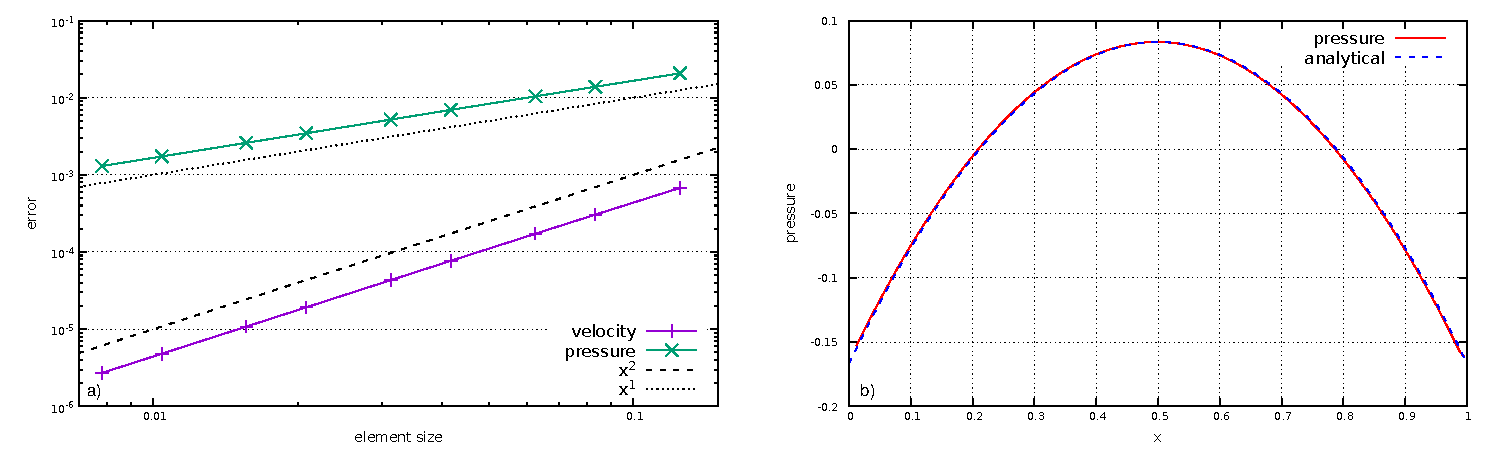
\includegraphics[width=\textwidth]{./Figures/errors.pdf}
\caption{Velocity and pressure error between the generated and the analytical solution as a function of element size.}
\label{fig:errors}
\end{figure}

\begin{figure}
\noindent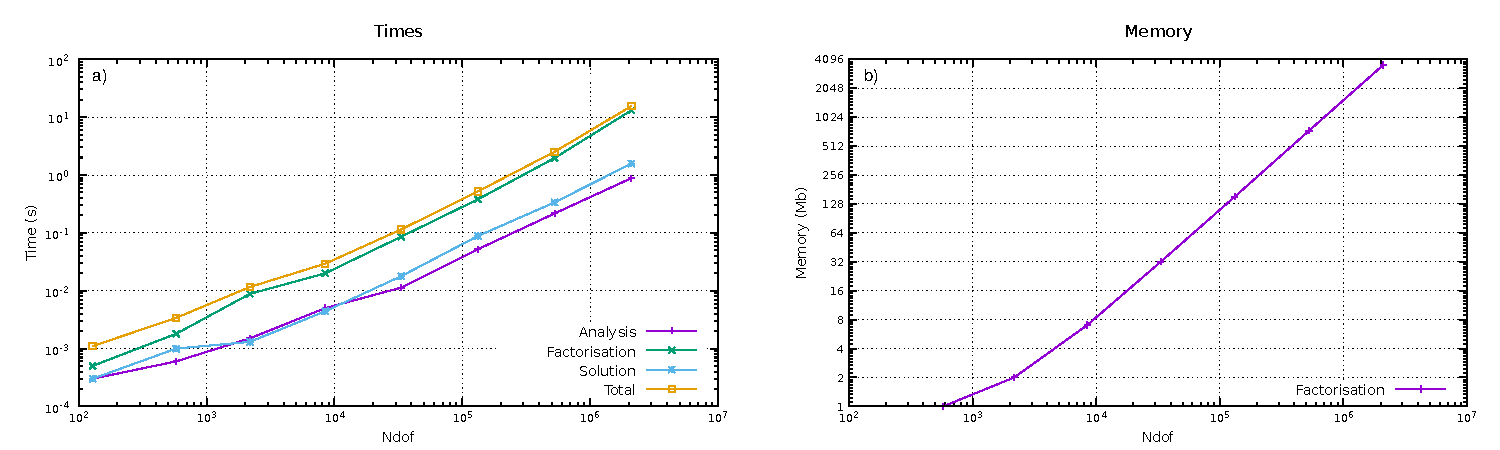
\includegraphics[width=\textwidth]{./Figures/MUMPS.pdf}
\caption{Panel a) Analysis, factorisation, solution and total solve times (panel a) and factorisation memory usage (panel b) as a function of the total number of degrees of freedom.}
\label{fig:MUMPS}
\end{figure}

\begin{figure}
\noindent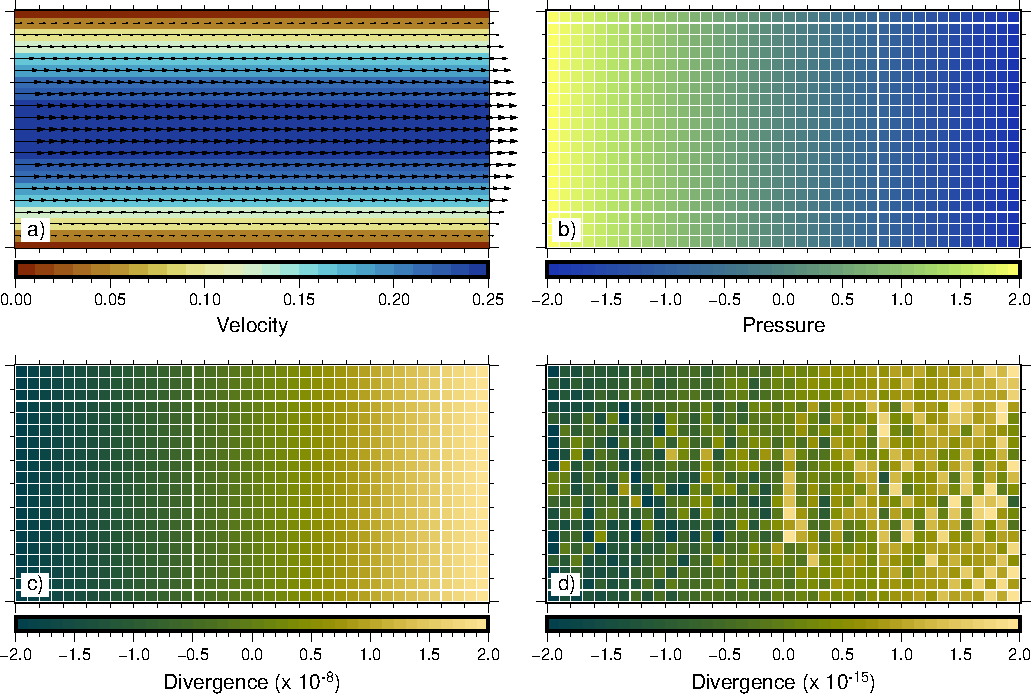
\includegraphics[width=\textwidth]{./Figures/Poiseuille.pdf}
\caption{Velocity field (panel a), pressure (panel b) and divergence velocity in case of the classic penalty method (no iterations) and after one Uzawa iteration (panel c and d, respectively).}
\label{fig:poiseuille}
\end{figure}

\begin{figure}
\noindent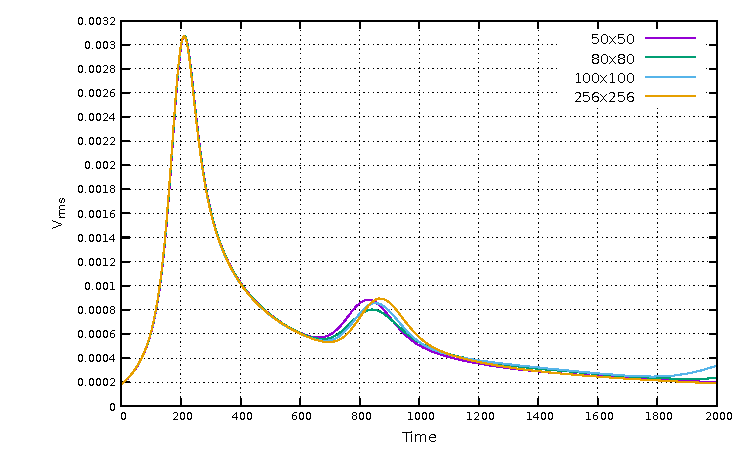
\includegraphics[width=\textwidth]{./Figures/RT.pdf}
\caption{Root-mean-square velocity ($v_{rms}$) in function of time for different resolution of the grid.}
\label{fig:RT}
\end{figure}

\begin{figure}
\noindent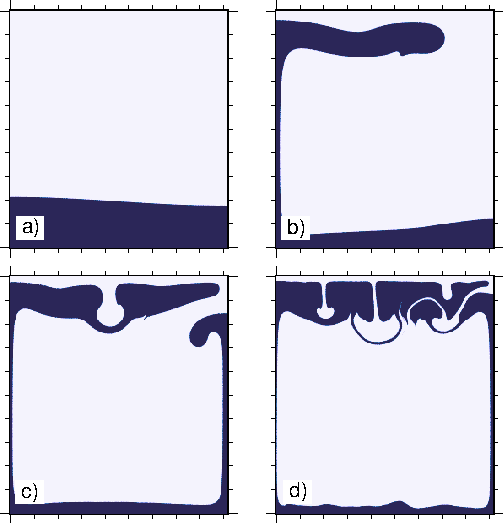
\includegraphics[width=\textwidth]{./Figures/Rayleigh.pdf}
\caption{Evolution of the Rayleigh-Taylor experiment for a grid of 256x256 elements at $t=0, 500, 1000$ and $2000$ (panels a, b, c and d, respectively).}
\label{fig:rayleigh}
\end{figure}

\begin{figure}
\noindent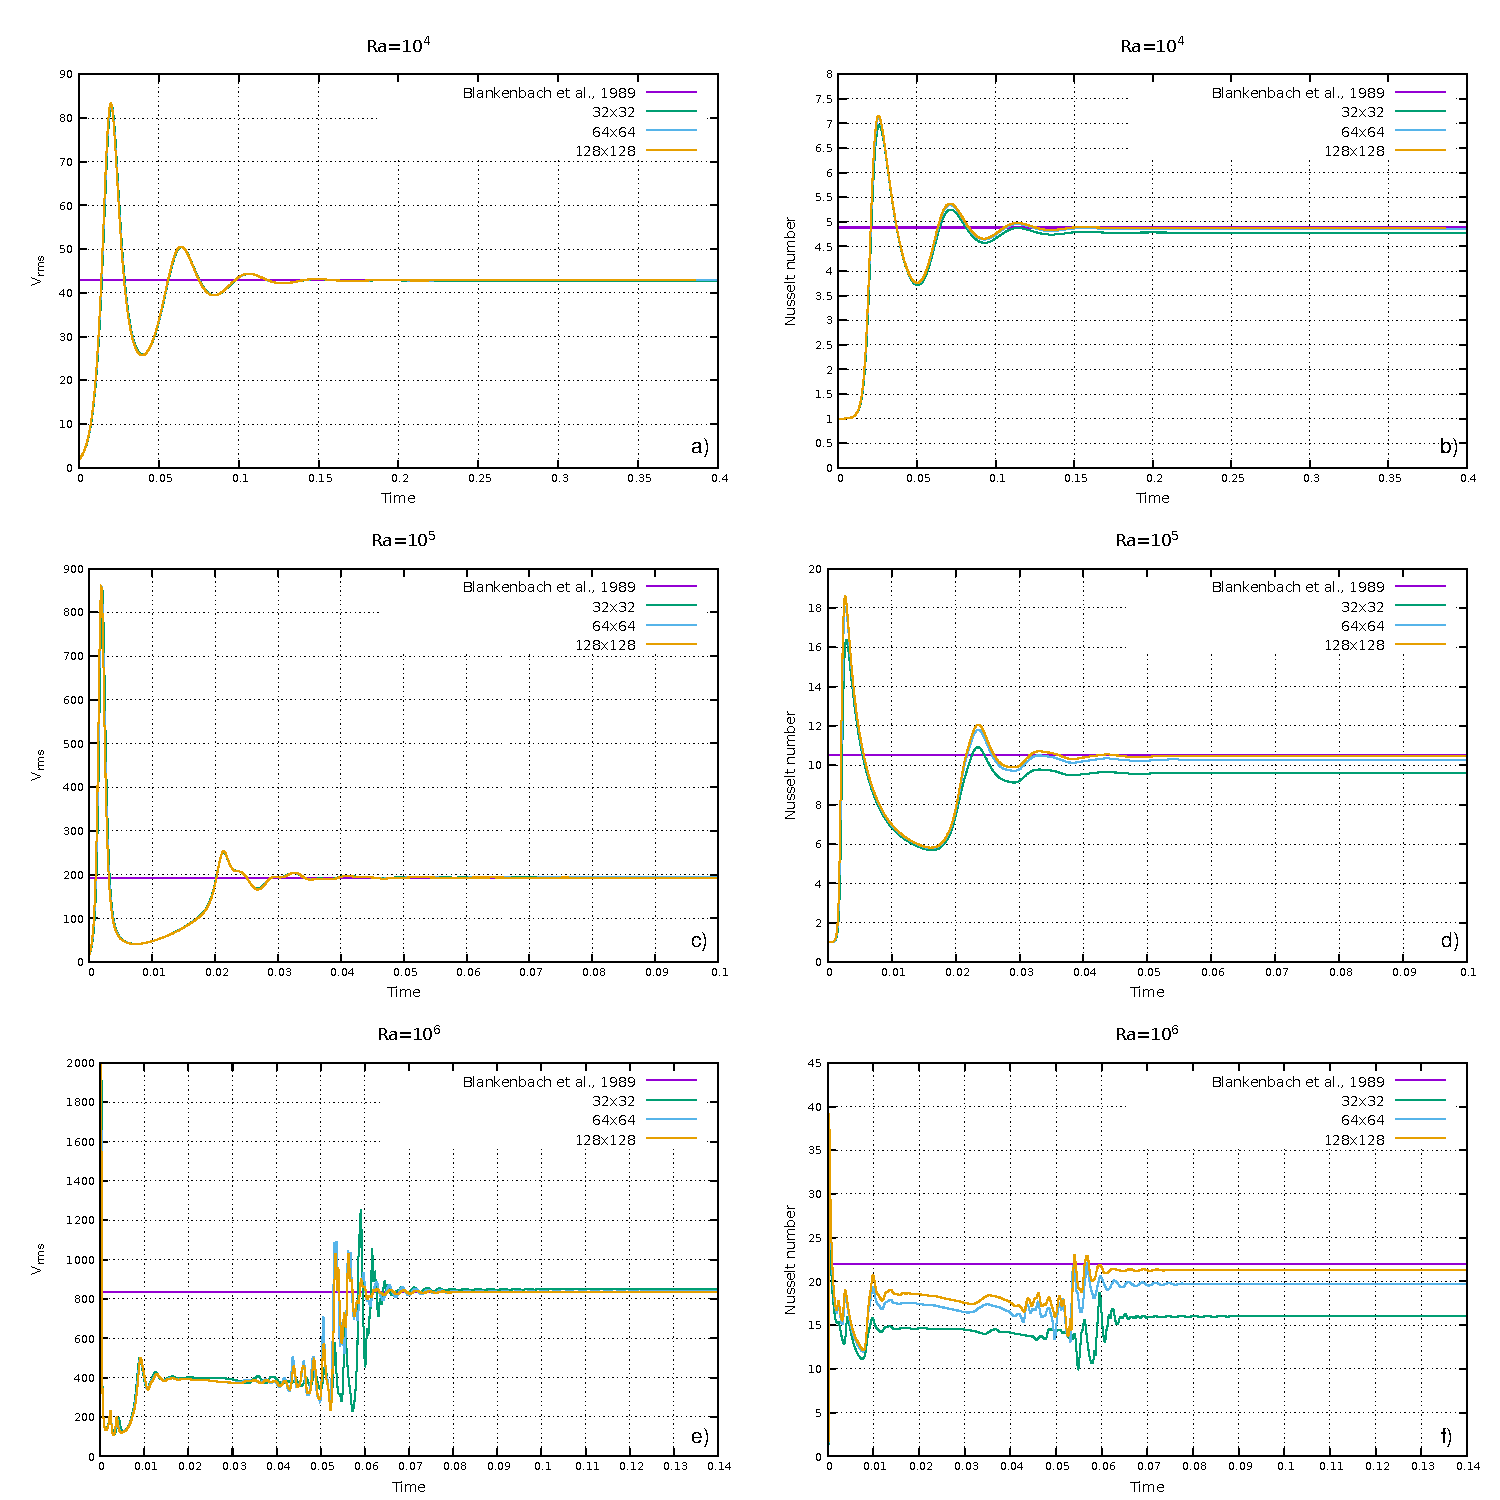
\includegraphics[width=\textwidth]{./Figures/Convection.pdf}
\caption{$v_{rms}$ (panels a, c and e) and $Nu$ (panels b, d and f) as function of time for different grid resolution. Panels a and b show the results for $Ra=10^4$; Panels c and d show the results for $Ra=10^5$; panels e and f show the results for $Ra=10^6$. Purple lines indicate the convergence values for the $v_{rms}$ and the $Nu$ from \citeA{Blankenbach1989} at the steady state.}
\label{fig:mantle}
\end{figure}

\begin{figure}
\noindent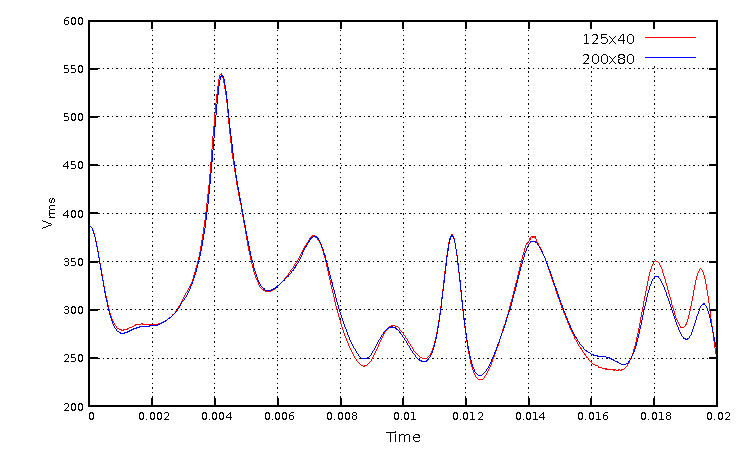
\includegraphics[width=\textwidth]{./Figures/Thin_Layer.pdf}
\caption{$v_{rms}$ as function of time for different grid resolution.}
\label{fig:thin}
\end{figure}

\begin{figure}
\noindent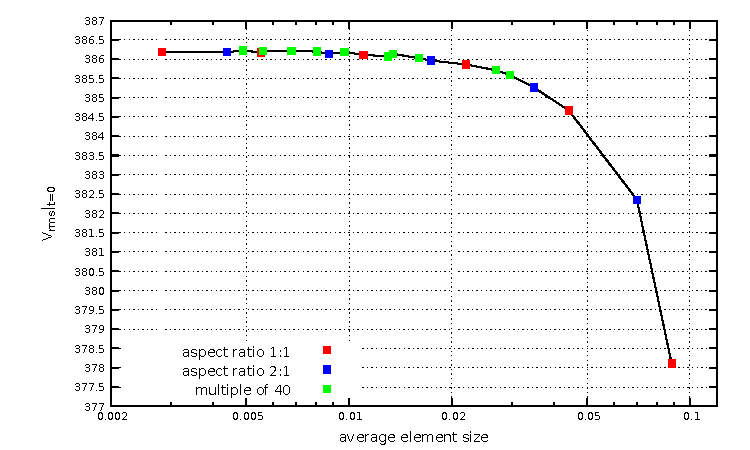
\includegraphics[width=\textwidth]{./Figures/Thin_Layer_Initial.pdf}
\caption{$v_{rms}$ at $t=0$ as function of the element size for different aspect ratios of the elements.}
\label{fig:thin_initial}
\end{figure}

\begin{figure}
\noindent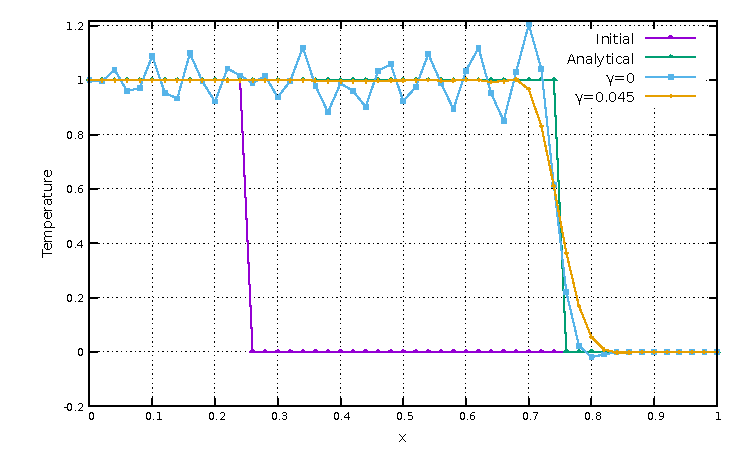
\includegraphics[width=\textwidth]{./Figures/Advection.pdf}
\caption{Temperature profile as function of \textit{x}. Purple line indicate the initial temperature profile; the green line inidicate the analytical temperature profile after 250 time steps; blue line indicate the temperature profile after 250 time steps in case of the classic Galerkin method ($\gamma=0$); orange line indicate the temperature profile after 250 time steps in case of the SUPG method ($\gamma=0.045$).}
\label{fig:advection}
\end{figure}

\begin{table}
\caption{List of benchmarks implemented for each feature of the code.}
\centering
\begin{tabular}{| l | l |}
\hline
 \textbf{Feature}  & \textbf{Benchmark}  \\
\hline
\hline
  Solver  & Stokes flow   \\
\hline
  Momentum and energy equations  & Poiseuille flow   \\
    & Instantaneous 2D sphere   \\
    & Rayleigh-Taylor experiment  \\
    & Mantle convection   \\
    & Thin layer   \\
    & Advection stabilisation   \\
\hline
  4th-order Runge-Kutta advection  & Zalesak disk   \\
\hline
  Large viscosity contrast  & Indenter   \\
    & Falling block   \\
\hline
  Non-linear visco-plasticity  & Indenter   \\
    & Brick   \\
    & Slab detachment   \\
\hline
  Shear and adiabatic heating  & ex. 9.4 in \citeA{Gerya2010b}   \\
\hline
  Free surface/sticky air  & Topography relaxation   \\
\hline
  Free surface stabilisation  & \citeA{Kaus2010a}, \citeA{Thieulot2014}   \\
\hline
  Markers chain  & Sinking ball   \\
  \hline
  Hydration  & Hydrated sinking ball   \\
\hline
\end{tabular}
\label{tab:list}
\end{table}

\begin{table}
\caption{Comparison between $v_{rms}$ and $Nu$ predicted by the code and same values reported in literature.}
\centering
\begin{tabular}{| l | l | l | l | l l l |}
\hline
  & & \citeA{Blankenbach1989} & \citeA{Thieulot2014} & 32x32 & 64x64 & 128x128  \\
\hline
\hline
 $Ra=10^4$ & $v_{rms}$ & $42.864947 \pm 0.000020$ & 42.867 & 42.83226 & 42.852793 & 42.861394  \\
           & $Nu$      & $4.884409 \pm 0.000010$  & 4.882  & 4.781297 & 4.857475  & 4.877573   \\
\hline
 $Ra=10^5$ & $v_{rms}$ & $193.21454 \pm 0.00010$  & 193.255& 193.872643 & 193.377472 & 193.252290  \\
           & $Nu$      & $10.534095 \pm 0.000010$ & 10.507 & 9.602514 & 10.270735  & 10.465629   \\
\hline
 $Ra=10^6$ & $v_{rms}$ & $833.98977 \pm 0.00020$  & 834.712& 848.091176 & 837.767911 & 834.945793  \\
           & $Nu$      & $21.972465 \pm 0.000020$ & 21.695 & 15.999266 & 19.703682  & 21.306939   \\
\hline
\end{tabular}
\label{tab:mantle}
\end{table}

%
%
% EXAMPLE FIGURES
% ---------------
% If you get an error about an unknown bounding box, try specifying the width and height of the figure with the natwidth and natheight options.
% \begin{figure}
%\setfigurenum{S1} %%You can change number for each figure if you want, not required. "S" prepended automatically.
% \noindent\includegraphics[natwidth=800px,natheight=600px]{samplefigure.eps}
%\caption{caption}
%\label{epsfiguresample}
%\end{figure}
%
%
% Giving latex a width will help it to scale the figure properly. A simple trick is to use \textwidth. Try this if large figures run off the side of the page.
% \begin{figure}
% \noindent\includegraphics[width=\textwidth]{anothersample.png}
%\caption{caption}
%\label{pngfiguresample}
%\end{figure}
%
%
%\begin{figure}
%\noindent\includegraphics[width=\textwidth]{athirdsample.pdf}
%\caption{A pdf test figure}
%\label{pdffiguresample}
%\end{figure}
%
% PDFLatex does not seem to be able to process EPS figures. You may want to try the epstopdf package.
%
%
% ---------------
% EXAMPLE TABLE
%
%\begin{table}
%\settablenum{S1} %%Change number for each table
%\caption{Time of the Transition Between Phase 1 and Phase 2\tablenotemark{a}}
%\centering
%\begin{tabular}{l c}
%\hline
% Run  & Time (min)  \\
%\hline
%  $l1$  & 260   \\
%  $l2$  & 300   \\
%  $l3$  & 340   \\
%  $h1$  & 270   \\
%  $h2$  & 250   \\
%  $h3$  & 380   \\
%  $r1$  & 370   \\
%  $r2$  & 390   \\
%\hline
%\end{tabular}
%\tablenotetext{a}{Footnote text here.}
%\end{table}
% ---------------
%
% EXAMPLE LARGE TABLE (UPLOADED SEPARATELY)
%\begin{table}
%\settablenum{S1} %%Change number for each table
%\caption{Time of the Transition Between Phase 1 and Phase 2\tablenotemark{a}}
%\end{table}


\end{document}

%%%%%%%%%%%%%%%%%%%%%%%%%%%%%%%%%%%%%%%%%%%%%%%%%%%%%%%%%%%%%%%

More Information and Advice:

%% ------------------------------------------------------------------------ %%
%
%  SECTION HEADS
%
%% ------------------------------------------------------------------------ %%

% Capitalize the first letter of each word (except for
% prepositions, conjunctions, and articles that are
% three or fewer letters).

% AGU follows standard outline style; therefore, there cannot be a section 1 without
% a section 2, or a section 2.3.1 without a section 2.3.2.
% Please make sure your section numbers are balanced.
% ---------------
% Level 1 head
%
% Use the \section{} command to identify level 1 heads;
% type the appropriate head wording between the curly
% brackets, as shown below.
%
%An example:
%\section{Level 1 Head: Introduction}
%
% ---------------
% Level 2 head
%
% Use the \subsection{} command to identify level 2 heads.
%An example:
%\subsection{Level 2 Head}
%
% ---------------
% Level 3 head
%
% Use the \subsubsection{} command to identify level 3 heads
%An example:
%\subsubsection{Level 3 Head}
%
%---------------
% Level 4 head
%
% Use the \subsubsubsection{} command to identify level 3 heads
% An example:
%\subsubsubsection{Level 4 Head} An example.
%
%% ------------------------------------------------------------------------ %%
%
%  IN-TEXT LISTS
%
%% ------------------------------------------------------------------------ %%
%
% Do not use bulleted lists; enumerated lists are okay.
% \begin{enumerate}
% \item
% \item
% \item
% \end{enumerate}
%
%% ------------------------------------------------------------------------ %%
%
%  EQUATIONS
%
%% ------------------------------------------------------------------------ %%

% Single-line equations are centered.
% Equation arrays will appear left-aligned.

Math coded inside display math mode \[ ...\]
 will not be numbered, e.g.,:
 \[ x^2=y^2 + z^2\]

 Math coded inside \begin{equation} and \end{equation} will
 be automatically numbered, e.g.,:
 \begin{equation}
 x^2=y^2 + z^2
 \end{equation}

% IF YOU HAVE MULTI-LINE EQUATIONS, PLEASE
% BREAK THE EQUATIONS INTO TWO OR MORE LINES
% OF SINGLE COLUMN WIDTH (20 pc, 8.3 cm)
% using double backslashes (\\).

% To create multiline equations, use the
% \begin{eqnarray} and \end{eqnarray} environment
% as demonstrated below.
\begin{eqnarray}
  x_{1} & = & (x - x_{0}) \cos \Theta \nonumber \\
        && + (y - y_{0}) \sin \Theta  \nonumber \\
  y_{1} & = & -(x - x_{0}) \sin \Theta \nonumber \\
        && + (y - y_{0}) \cos \Theta.
\end{eqnarray}

%If you don't want an equation number, use the star form:
%\begin{eqnarray*}...\end{eqnarray*}

% Break each line at a sign of operation
% (+, -, etc.) if possible, with the sign of operation
% on the new line.

% Indent second and subsequent lines to align with
% the first character following the equal sign on the
% first line.

% Use an \hspace{} command to insert horizontal space
% into your equation if necessary. Place an appropriate
% unit of measure between the curly braces, e.g.
% \hspace{1in}; you may have to experiment to achieve
% the correct amount of space.


%% ------------------------------------------------------------------------ %%
%
%  EQUATION NUMBERING: COUNTER
%
%% ------------------------------------------------------------------------ %%

% You may change equation numbering by resetting
% the equation counter or by explicitly numbering
% an equation.

% To explicitly number an equation, type \eqnum{}
% (with the desired number between the brackets)
% after the \begin{equation} or \begin{eqnarray}
% command.  The \eqnum{} command will affect only
% the equation it appears with; LaTeX will number
% any equations appearing later in the manuscript
% according to the equation counter.
%

% If you have a multiline equation that needs only
% one equation number, use a \nonumber command in
% front of the double backslashes (\\) as shown in
% the multiline equation above.

%% ------------------------------------------------------------------------ %%
%
%  SIDEWAYS FIGURE AND TABLE EXAMPLES
%
%% ------------------------------------------------------------------------ %%
%
% For tables and figures, add \usepackage{rotating} to the paper and add the rotating.sty file to the folder.
% AGU prefers the use of {sidewaystable} over {landscapetable} as it causes fewer problems.
%
% \begin{sidewaysfigure}
% \includegraphics[width=20pc]{samplefigure.eps}
% \caption{caption here}
% \label{label_here}
% \end{sidewaysfigure}
%
%
%
% \begin{sidewaystable}
% \caption{}
% \begin{tabular}
% Table layout here.
% \end{tabular}
% \end{sidewaystable}
%
%
\grid
